\documentclass[11pt,a4paper]{article}

\usepackage[margin=2.3cm]{geometry}
\usepackage{amsmath,amssymb,amsthm}
\usepackage{graphicx}
\usepackage{booktabs}
\usepackage{float}
\usepackage{caption}
\usepackage{subcaption}
\usepackage{enumitem}
\usepackage{xcolor}
\usepackage[colorlinks=true,linkcolor=blue!50!black,citecolor=blue!50!black,urlcolor=blue!50!black]{hyperref}

\graphicspath{{../results/figures/}}
\captionsetup{font=small,labelfont=bf}
\setlength{\parskip}{0.35em}
\newtheorem{proposition}{Proposition}

\title{\textbf{Auctions and the VCG Mechanism:\\A Simulation Study of Incentive Compatibility}\\[0.4em]
\large Assignment 4}
\author{Vaibhav Garg \and Aditya Bansal \and Meet Tilala}
\date{November 2026}

\begin{document}
\maketitle

\begin{abstract}
We study three mechanisms by simulation and compare every result with its closed-form prediction.
In the second-price sealed-bid auction, truthful bidding maximises bidder~1's utility in all
18 random-rival settings (values $v\in\{0.2,0.5,0.8\}$, three rival strategies, one or two rivals)
and in all 36 fixed-rival-bid profiles we tested.
In the first-price auction with $n=2,3,4$ bidders, bidder~1's best multiplier is
$k^\ast=(n-1)/n$, and its expected utility there is $1/(n(n+1))$, exactly the symmetric
equilibrium. The winner, however, could have paid less and still won in every simulated auction,
and in 95--99\% of auctions by more than one bid increment.
Finally, the VCG mechanism for buying the cheapest $A\to F$ path reproduces the textbook outcome:
path $A$--$B$--$E$--$F$ with payments $AB=4$, $BE=2$, $EF=3$ and $0$ to every other edge.
A sweep of misreported costs from 0 to 10 shows that no edge ever gains by lying.
\end{abstract}

%=====================================================================
\section{Introduction}
%=====================================================================
A mechanism is \emph{dominant-strategy incentive compatible} (DSIC) if reporting one's
private information truthfully is optimal whatever the other agents do. The Vickrey
(second-price) auction~\cite{vickrey1961} and its generalisation, the Vickrey--Clarke--Groves
(VCG) mechanism~\cite{clarke1971,groves1973}, are the canonical DSIC mechanisms. The first-price
auction is not DSIC: a bidder's best bid depends on what it believes the others will bid.

The assignment asks us to check these properties empirically:
\begin{enumerate}[leftmargin=*,itemsep=0.2em]
  \item \textbf{Second-price auction.} Bidder~1 has value $v\in\{0.2,0.5,0.8\}$. Each rival draws a value from $U[0,1]$ and follows one of three strategies: (a) bid truthfully, (b) bid half its value, (c) bid a fresh $U[0,1]$ number and ignore its value.
  \begin{enumerate}[label=\Alph*.,itemsep=0.1em]
    \item For each bid $b=0.00,0.01,\dots,1.00$, simulate at least 100{,}000 auctions and plot bidder~1's average utility (9 plots).
    \item Fix the rival bid at $0.1$, $0.4$ and $0.9$, and confirm that $b=v$ maximises utility.
    \item Repeat A and B with two rivals who use the same strategy.
  \end{enumerate}
  \item \textbf{First-price auction with $n$ bidders.} Bidders $2,\dots,n$ bid $\frac{n-1}{n}v$. Bidder~1 bids $k\,v$ with $k\in[0.1,2.0]$. Estimate bidder~1's expected utility for each $k$, and measure the fraction of auctions in which the winner could have paid less and still won, for $n=2,3,4$.
  \item \textbf{VCG for a cheapest path.} Each edge of the network in Figure~7.3 of the textbook is an agent with a private cost. Reproduce the chosen path $ABEF$ and its payments, then sweep one on-path and one off-path edge's reported cost from 0 to 10 in steps of 0.5.
\end{enumerate}

Section~\ref{sec:part1} covers the second-price auction, Section~\ref{sec:part2} the first-price
auction and Section~\ref{sec:part3} the VCG mechanism. Section~\ref{sec:impl} describes the
implementation, and Section~\ref{sec:conc} concludes.

%=====================================================================
\section{Part 1: Second-Price Sealed-Bid Auction}\label{sec:part1}
%=====================================================================
\subsection{Model}
Bidder~1 has a fixed value $v$ and bids $b$. Let $R$ be the highest rival bid. The highest bid
wins and pays the highest competing bid, so
\begin{equation}
u_1(b) = (v - R)\,\mathbf{1}\{b > R\}.
\end{equation}
Ties ($b=R$) are broken uniformly at random among the tied bidders. They only occur in Part~B,
where rival bids are fixed. If $R$ has density $f_R$, the expected utility is
\begin{equation}\label{eq:spa}
U(b) = \mathbb{E}[u_1(b)] = \int_0^{b} (v-r)\,f_R(r)\,dr,
\qquad U'(b) = (v-b)\,f_R(b).
\end{equation}
Since $U'(b)\ge 0$ for $b<v$ and $U'(b)\le 0$ for $b>v$, the bid $b=v$ maximises $U$ for
\emph{every} rival bid distribution. Truthful bidding is therefore a dominant strategy.

The three rival strategies induce the following bid distributions:
\begin{itemize}[itemsep=0.1em]
  \item \textbf{Truthful:} each rival bids $V_j\sim U[0,1]$.
  \item \textbf{Half:} each rival bids $V_j/2\sim U[0,0.5]$.
  \item \textbf{Random:} each rival bids an independent $U[0,1]$ draw.
\end{itemize}
The random strategy ignores the value, but its bids have the same distribution as truthful bids.
Bidder~1 only ever sees bids, so the two strategies give identical utility curves.
Evaluating~\eqref{eq:spa} gives the closed forms in Table~\ref{tab:closed}, which we plot next to
every simulated curve.

\begin{table}[!htbp]
\centering
\caption{Closed-form expected utility $U(b)$ of bidder~1 in the second-price auction.}
\label{tab:closed}
\begin{tabular}{lll}
\toprule
Rival strategy & One rival & Two rivals \\
\midrule
Truthful / random & $vb - b^2/2$ & $vb^2 - \tfrac{2}{3}b^3$ \\
Half ($x=\min(b,0.5)$) & $2vx - x^2$ & $4vx^2 - \tfrac{8}{3}x^3$ \\
\bottomrule
\end{tabular}
\end{table}

\subsection{Experimental setup}
For every combination of $v$, rival strategy and number of rivals, we simulate 100{,}000
auctions for each of the 101 bids $b=0.00,\dots,1.00$. Every bid faces the same 100{,}000 rival
draws (\emph{common random numbers}). This is a standard variance-reduction technique: the
comparison between two bids then reflects only the change in bid, not sampling noise. Near the
peak, neighbouring bids differ in expected utility by about $5\times10^{-5}$. That gap is far
smaller than the standard error of an individual mean (about $5\times10^{-4}$), so without common
draws the empirical argmax would wander around $v$ by chance.

\subsection{Results for Part A (one rival)}
Figure~\ref{fig:p1a1} shows the nine required plots. In every panel the simulated curve lies on
the closed form; the largest absolute deviation over all bids is $0.0023$. The curve peaks at
$b=v$, marked by the red dot.

\begin{figure}[!htbp]
\centering
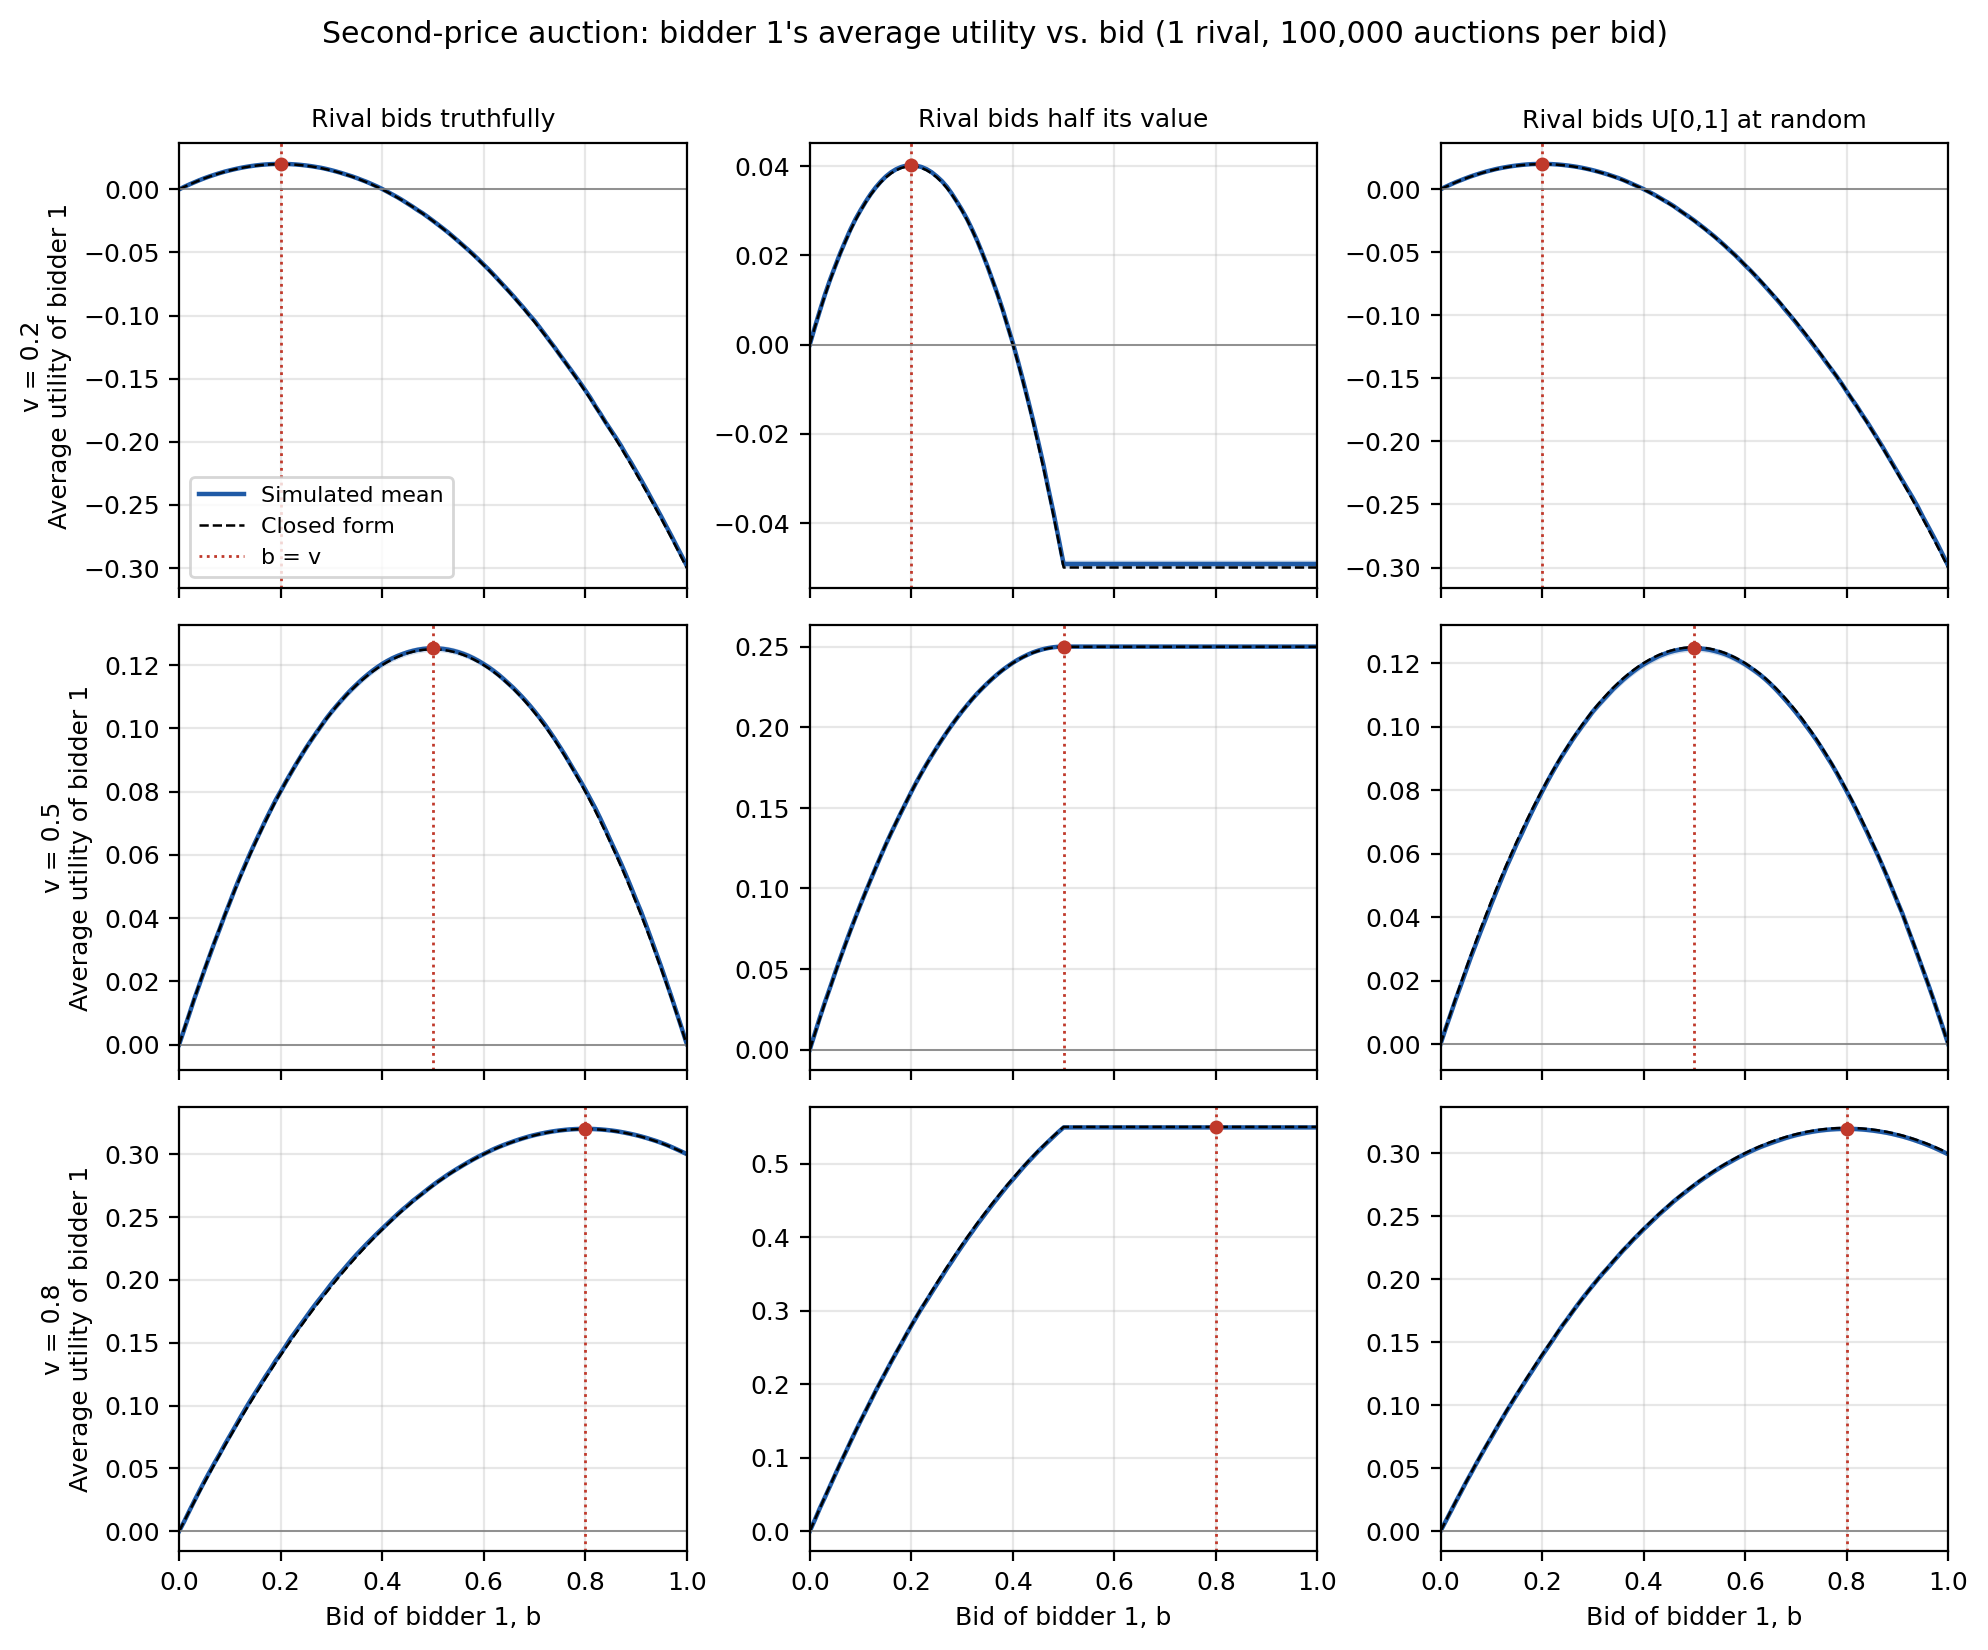
\includegraphics[width=0.97\linewidth]{part1A_grid_1rival.png}
\caption{Part~A, one rival. Average utility of bidder~1 against its bid, for each value $v$
(rows) and rival strategy (columns). Blue: simulation (100{,}000 auctions per bid, 95\%
confidence band). Dashed: closed form. Dotted red: $b=v$.}
\label{fig:p1a1}
\end{figure}

\begin{table}[!htbp]
\centering
\caption{Part~A and Part~C-A summary. ``Optimal bids'' is the set of bids whose simulated utility equals the maximum. $\hat U(v)$ is the simulated utility at $b=v$ and $U(v)$ the closed form.}
\label{tab:p1a}
\small
\begin{tabular}{cl ccc ccc}
\toprule
& & \multicolumn{3}{c}{One rival} & \multicolumn{3}{c}{Two rivals} \\
\cmidrule(lr){3-5}\cmidrule(lr){6-8}
$v$ & Rival strategy & Optimal bids & $\hat U(v)$ & $U(v)$ & Optimal bids & $\hat U(v)$ & $U(v)$ \\
\midrule
0.2 & Truthful & 0.20 & 0.0202 & 0.0200 & 0.20 & 0.0026 & 0.0027 \\
0.2 & Half     & 0.20 & 0.0402 & 0.0400 & 0.20 & 0.0106 & 0.0107 \\
0.2 & Random   & 0.20 & 0.0202 & 0.0200 & 0.20 & 0.0026 & 0.0027 \\
0.5 & Truthful & 0.50 & 0.1253 & 0.1250 & 0.50 & 0.0414 & 0.0417 \\
0.5 & Half     & [0.50, 1.00] & 0.2502 & 0.2500 & [0.50, 1.00] & 0.1670 & 0.1667 \\
0.5 & Random   & 0.50 & 0.1247 & 0.1250 & 0.50 & 0.0419 & 0.0417 \\
0.8 & Truthful & 0.80 & 0.3202 & 0.3200 & 0.80 & 0.1705 & 0.1707 \\
0.8 & Half     & [0.50, 1.00] & 0.5493 & 0.5500 & [0.50, 1.00] & 0.4671 & 0.4667 \\
0.8 & Random   & 0.80 & 0.3193 & 0.3200 & 0.80 & 0.1707 & 0.1707 \\
\bottomrule
\end{tabular}
\end{table}

\paragraph{Do the plots help bidder 1 choose its strategy?} Yes. Table~\ref{tab:p1a} shows that
$b=v$ is optimal in all nine cases, so bidder~1 should bid its value \emph{without knowing which
strategy the rival uses}. The plots also show why deviations hurt:
\begin{itemize}[itemsep=0.1em]
  \item \textbf{Underbidding} ($b<v$) loses auctions that would have been profitable, i.e.\ those with $b<R<v$.
  \item \textbf{Overbidding} ($b>v$) wins auctions at a loss, i.e.\ those with $v<R<b$. With $v=0.2$ and a truthful rival, bidding $b=1$ gives an expected utility of $-0.30$.
\end{itemize}
When the rival bids half its value, $R<0.5$ always. For $v\ge 0.5$ every bid $b\ge 0.5$ then wins
every auction and earns the same utility, so the curve is flat. Truthful bidding is still optimal
there; it is weakly rather than strictly better. The truthful and random columns are identical, as
predicted, because both strategies produce $U[0,1]$ bids.

\subsection{Results for Part B (fixed rival bid)}
When the rival bid is a fixed number $r$, $u_1(b)=v-r$ if $b>r$, $(v-r)/2$ if $b=r$, and $0$
otherwise. Figure~\ref{fig:p1b1} and Table~\ref{tab:p1b} show that $b=v$ attains the maximum
utility in all nine $(v,r)$ combinations:
\begin{itemize}[itemsep=0.1em]
  \item If $v>r$, every bid above $r$ wins and earns $v-r$, and $b=v$ is one of them.
  \item If $v<r$, every bid below $r$ loses and earns $0$, again including $b=v$, while any bid above $r$ earns the negative amount $v-r$.
\end{itemize}
Truthful bidding therefore needs no knowledge of $r$: it lands in the optimal set automatically.

\begin{figure}[!htbp]
\centering
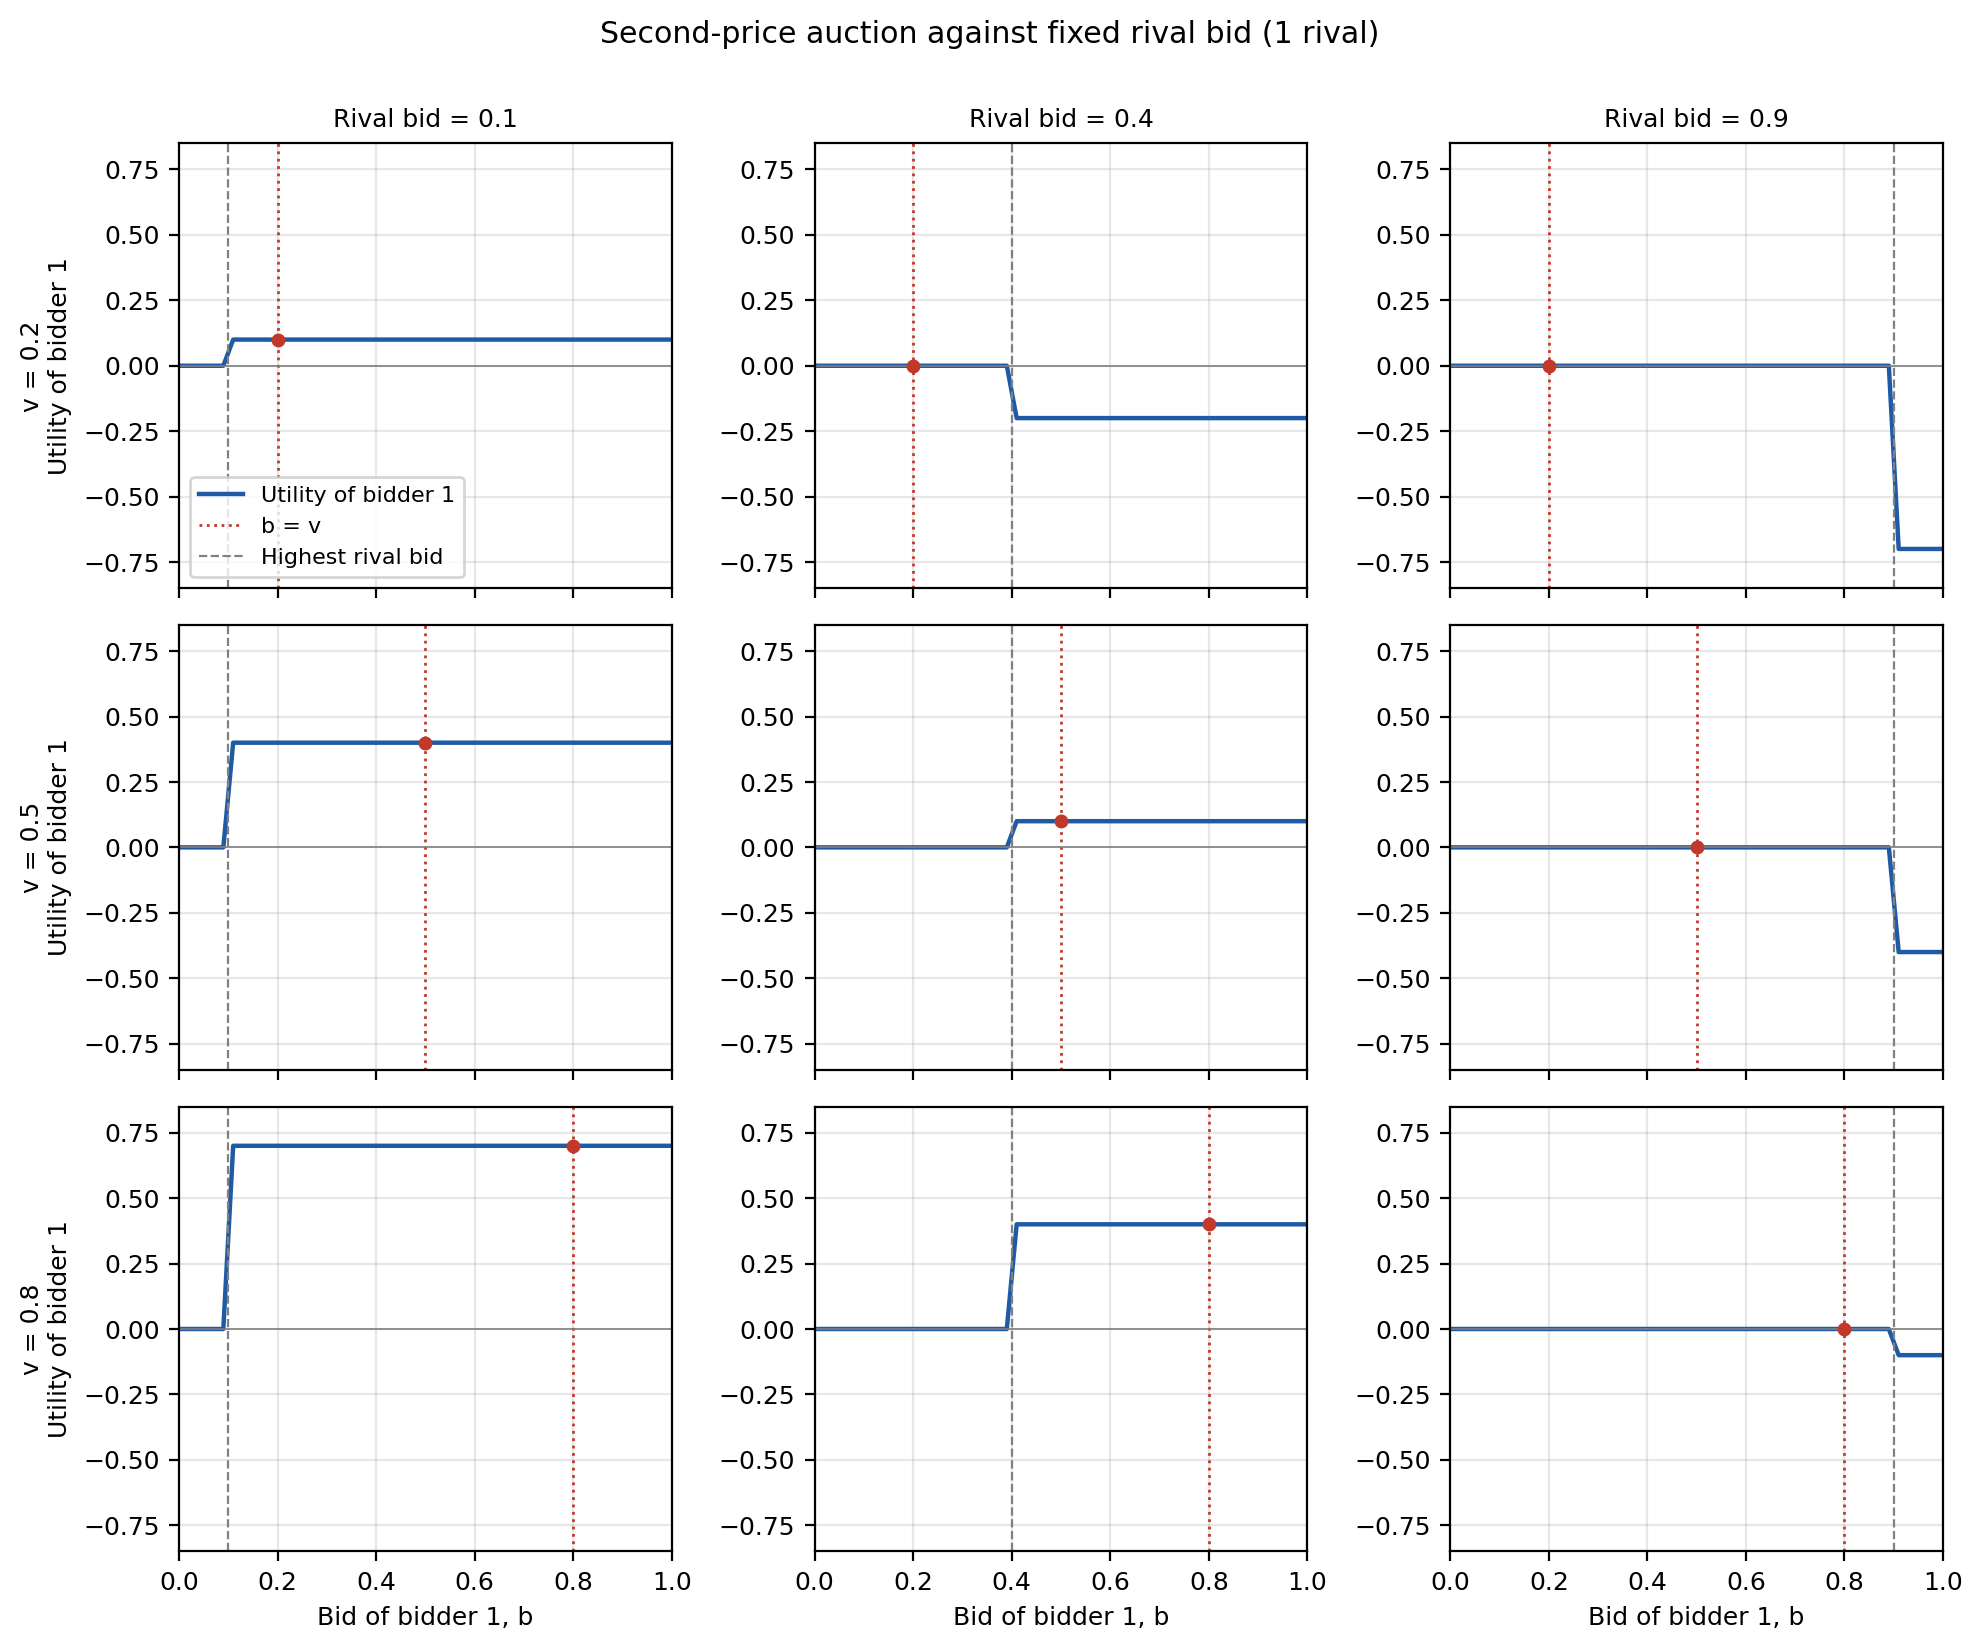
\includegraphics[width=0.92\linewidth]{part1B_grid_1rival.png}
\caption{Part~B, one rival with a fixed bid $r\in\{0.1,0.4,0.9\}$. The red dot at $b=v$ is
always on the highest level of the step function.}
\label{fig:p1b1}
\end{figure}

\begin{table}[!htbp]
\centering
\caption{Part~B and Part~C-B: exact utility against fixed rival bids. With two rivals we tested
all 9 ordered pairs from $\{0.1,0.4,0.9\}^2$. Utility depends only on the highest rival bid $m$,
and the rows below hold for every pair with that maximum. The range of optimal bids is on the
$0.01$ grid. A bid exactly equal to $m$ ties and earns only a share of $v-m$.}
\label{tab:p1b}
\small
\begin{tabular}{cc ccc c}
\toprule
$v$ & Highest rival bid $m$ & $u_1(b=v)$ & $\max_b u_1(b)$ & Optimal bids & $b=v$ optimal? \\
\midrule
0.2 & 0.1 & $+0.10$ & $+0.10$ & $[0.11,1.00]$ & yes \\
0.2 & 0.4 & $0.00$ & $0.00$ & $[0.00,0.39]$ & yes \\
0.2 & 0.9 & $0.00$ & $0.00$ & $[0.00,0.89]$ & yes \\
0.5 & 0.1 & $+0.40$ & $+0.40$ & $[0.11,1.00]$ & yes \\
0.5 & 0.4 & $+0.10$ & $+0.10$ & $[0.41,1.00]$ & yes \\
0.5 & 0.9 & $0.00$ & $0.00$ & $[0.00,0.89]$ & yes \\
0.8 & 0.1 & $+0.70$ & $+0.70$ & $[0.11,1.00]$ & yes \\
0.8 & 0.4 & $+0.40$ & $+0.40$ & $[0.41,1.00]$ & yes \\
0.8 & 0.9 & $0.00$ & $0.00$ & $[0.00,0.89]$ & yes \\
\bottomrule
\end{tabular}
\end{table}

\subsection{Results for Part C (two rivals)}
With two rivals, $R=\max(B_2,B_3)$ is the highest of two bids. This changes the shape of $U(b)$
but not its maximiser, because the argument after~\eqref{eq:spa} holds for any $f_R$.
Figure~\ref{fig:p1a2} repeats Part~A. The utility levels fall, since bidder~1 wins less often
and pays more when it wins: for $v=0.8$ against truthful rivals, $U(v)$ drops from $0.320$ to
$0.171$. The peak, however, stays at $b=v$ in all nine panels (Table~\ref{tab:p1a}).
Figure~\ref{fig:p1b2} repeats Part~B for three representative pairs of fixed rival bids; all 27
$(v,\text{pair})$ combinations give $b=v$ as a best response (Table~\ref{tab:p1b}).

\begin{figure}[!htbp]
\centering
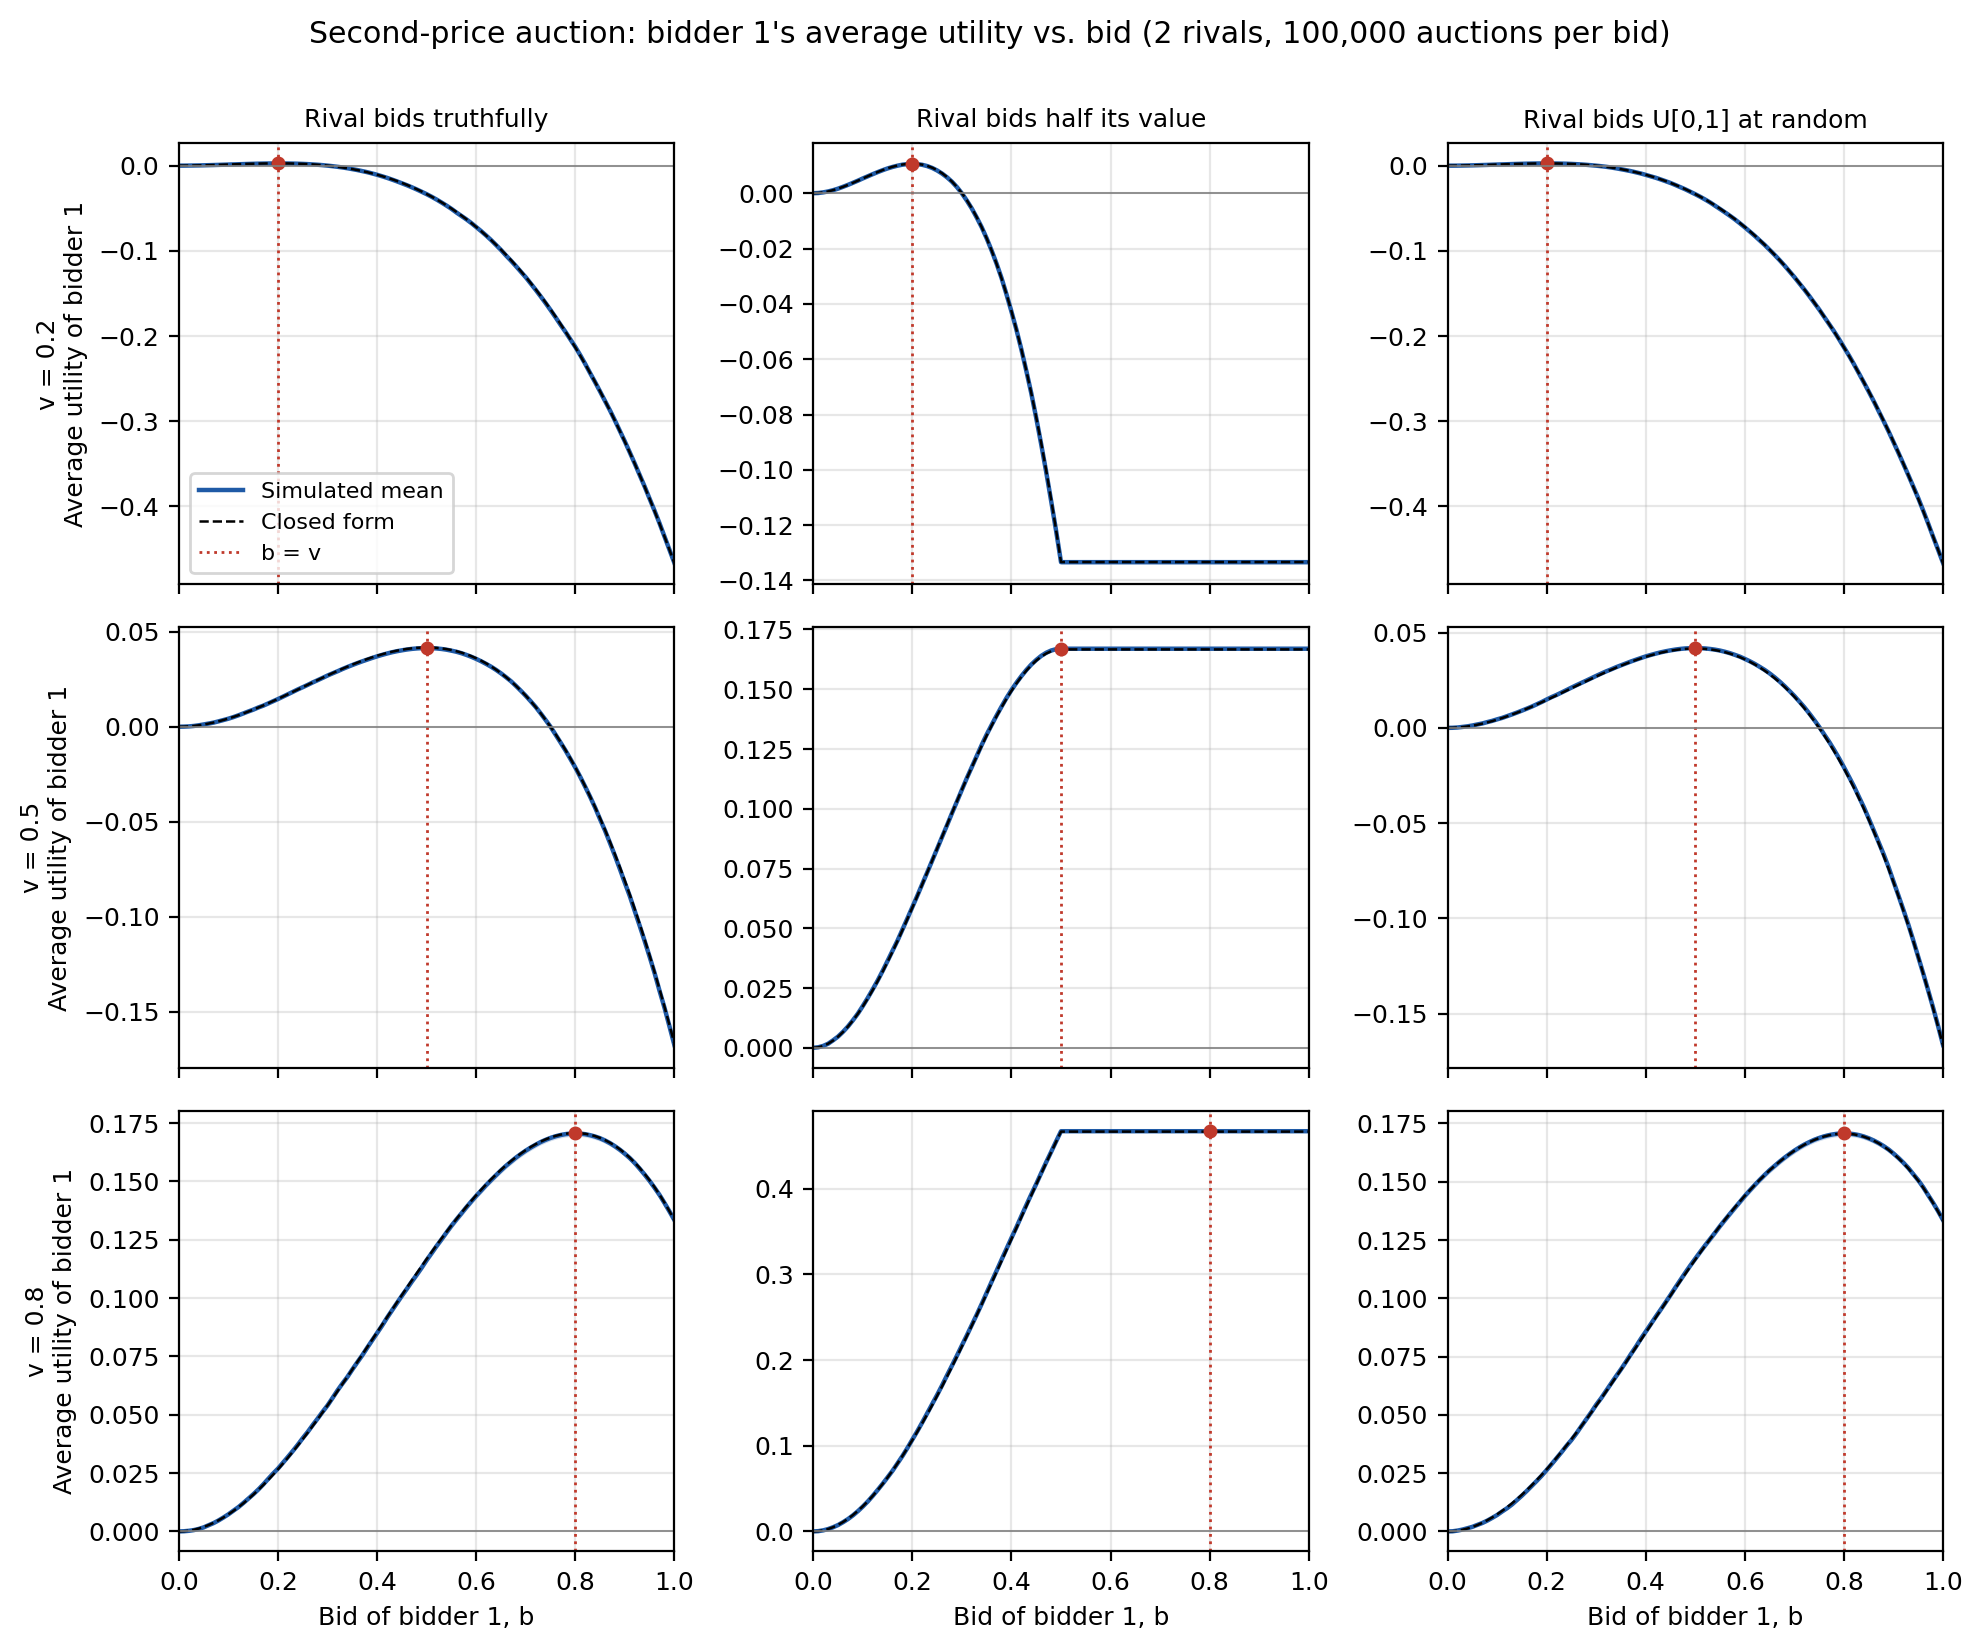
\includegraphics[width=0.97\linewidth]{part1A_grid_2rival.png}
\caption{Part~C-A, two rivals using the same strategy. Same layout as Figure~\ref{fig:p1a1}.}
\label{fig:p1a2}
\end{figure}

\begin{figure}[!htbp]
\centering
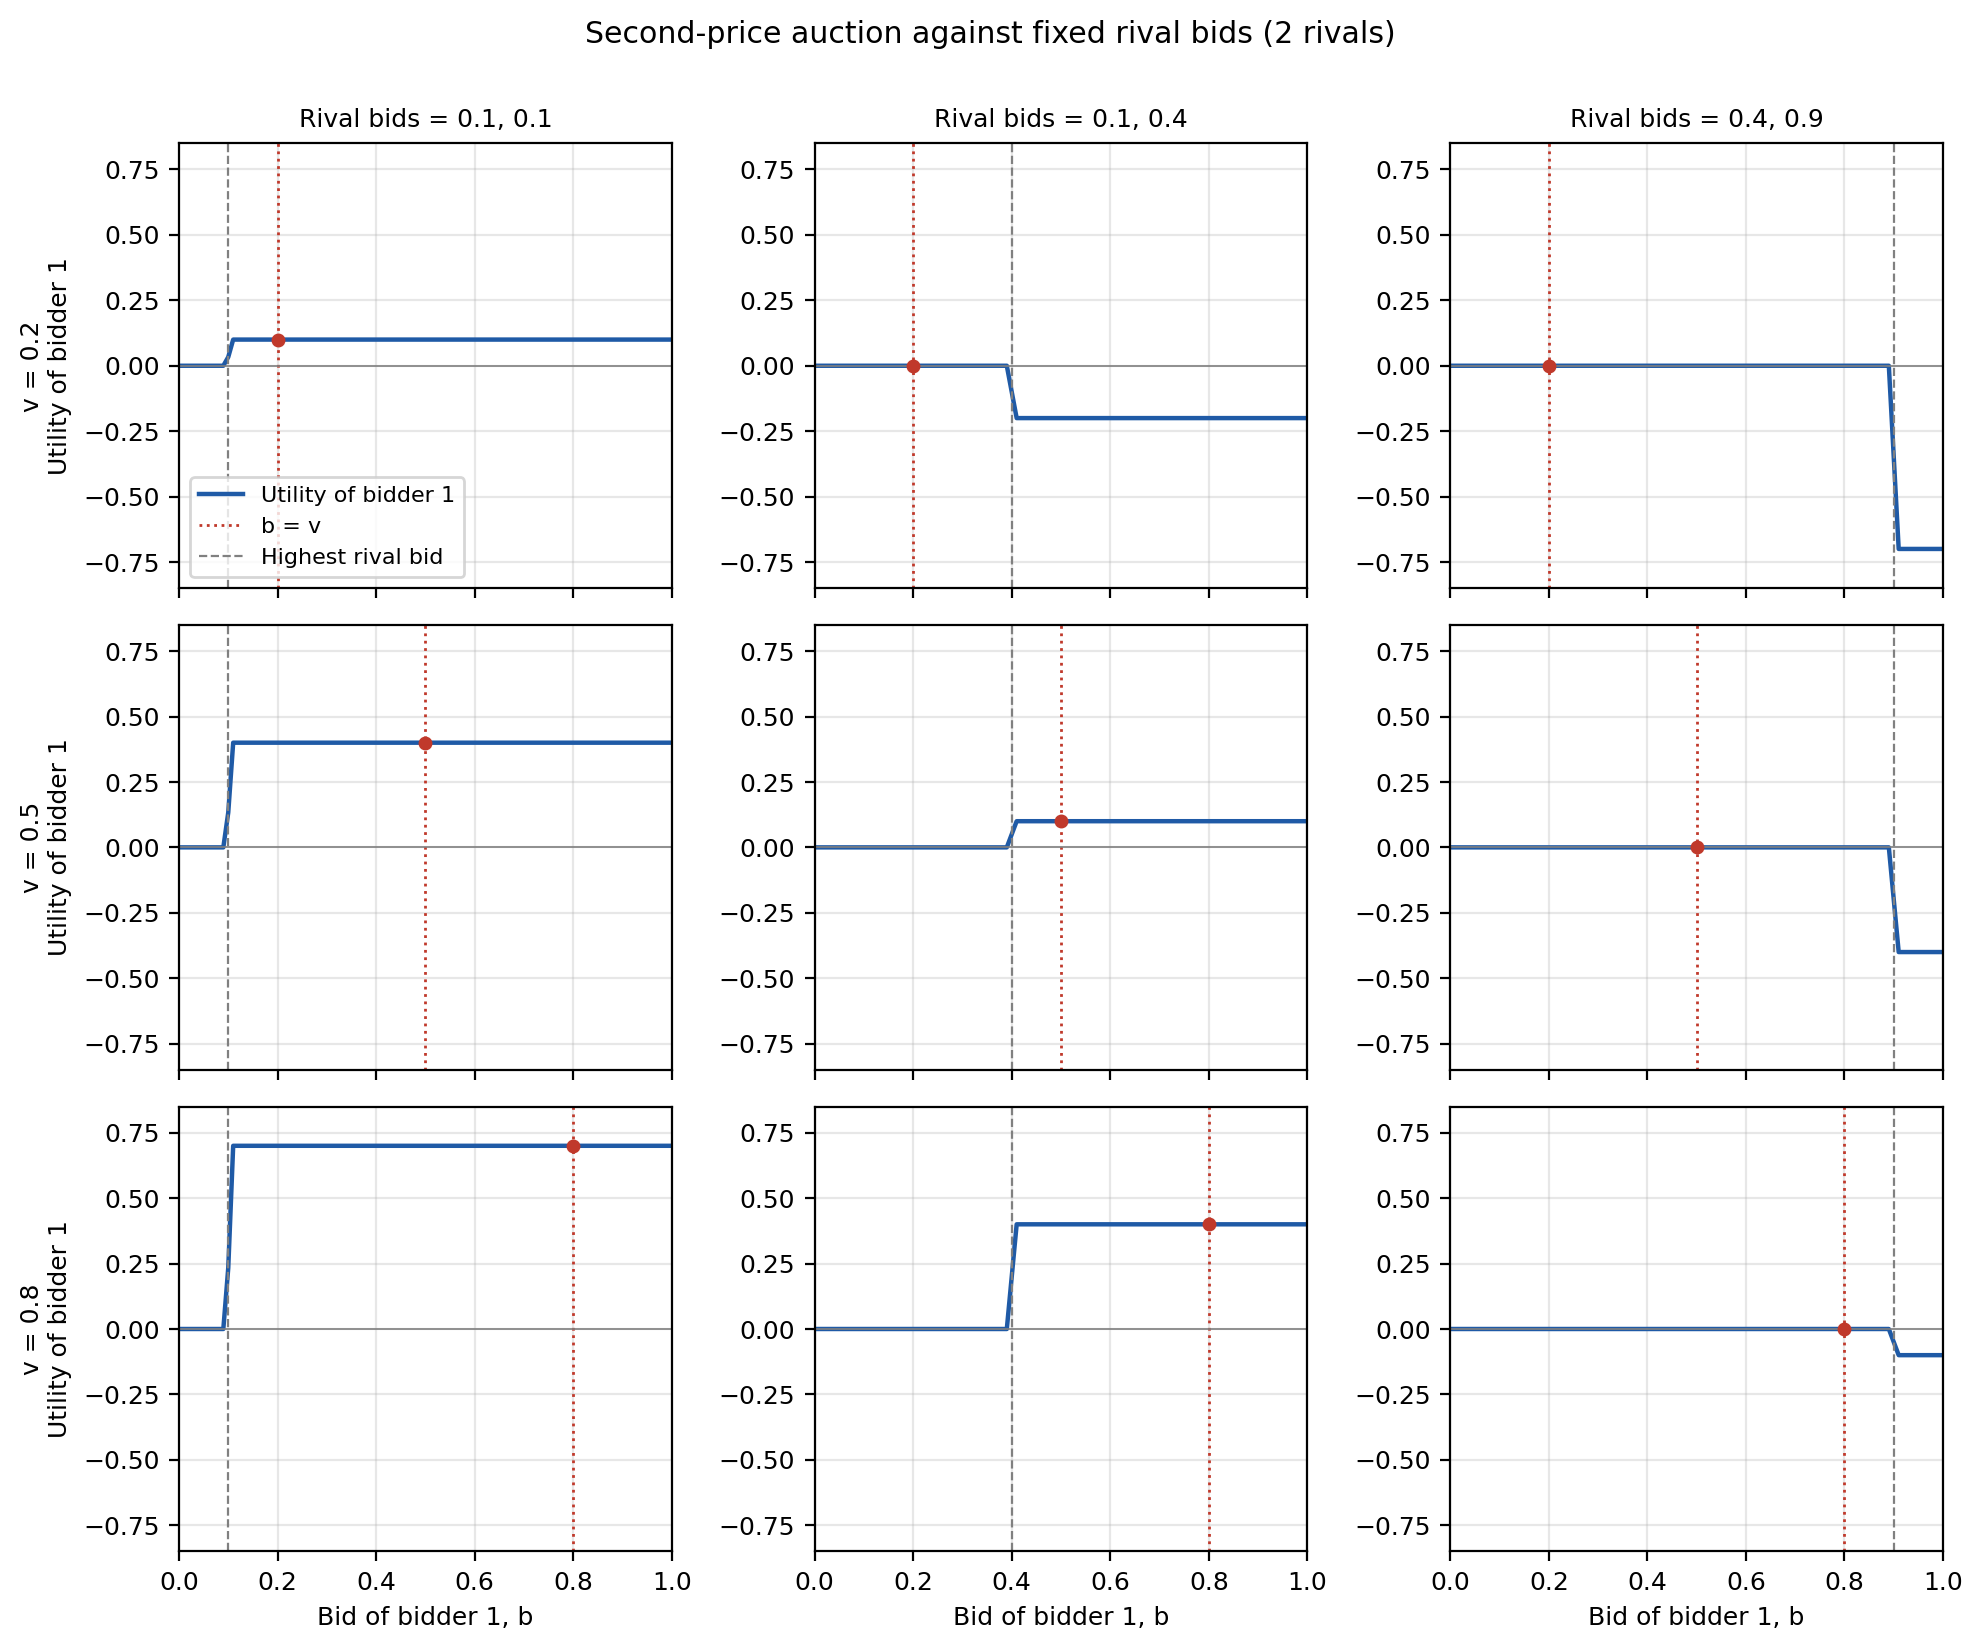
\includegraphics[width=0.92\linewidth]{part1B_grid_2rival.png}
\caption{Part~C-B, two rivals with fixed bids. Shown: pairs $(0.1,0.1)$, $(0.1,0.4)$ and
$(0.4,0.9)$, whose highest bids are $0.1$, $0.4$ and $0.9$.}
\label{fig:p1b2}
\end{figure}

%=====================================================================
\section{Part 2: First-Price Auction with $n$ Bidders}\label{sec:part2}
%=====================================================================
\subsection{Model and closed form}
All $n$ values are i.i.d.\ $U[0,1]$. The highest bid wins and the winner pays \emph{its own}
bid. In the symmetric Bayes--Nash equilibrium every bidder bids
$\beta(v)=\frac{n-1}{n}v$~\cite{krishna2009}. Bidders $2,\dots,n$ play $\beta$, and bidder~1 bids
$k\,v_1$. Bidder~1 wins iff $k v_1 > \frac{n-1}{n}\max_{j\ge2} v_j$, so
\begin{equation}
U(k) = \int_0^1 (1-k)\,v\,\min\!\Big(1,\tfrac{kvn}{n-1}\Big)^{n-1}dv.
\end{equation}
For $k\le\frac{n-1}{n}$ the minimum is never binding, and
\begin{equation}\label{eq:fpa}
U(k) = \frac{(1-k)\,k^{n-1}}{n+1}\Big(\frac{n}{n-1}\Big)^{n-1}.
\end{equation}
Setting $\frac{d}{dk}\big[(1-k)k^{n-1}\big]=0$ gives $k^\ast=\frac{n-1}{n}$, with
$U(k^\ast)=\frac{1}{n(n+1)}$.

For $k>\frac{n-1}{n}$, write $a=\frac{kn}{n-1}>1$. Then
$U(k)=(1-k)\big[\frac{1}{(n+1)a^2}+\frac{1}{2}\big(1-\frac{1}{a^2}\big)\big]$, which is smaller
than $U(k^\ast)$ and negative for $k>1$. So deviating from the equilibrium bid never helps
bidder~1, which confirms that $\beta$ is a best response to itself.

\subsection{Experimental setup}
For each $n\in\{2,3,4\}$ we draw 200{,}000 auctions and reuse them for every $k$ (common random
numbers). The grid is $k=0.10,0.15,\dots,2.00$, plus $k=2/3$ so that every equilibrium multiplier
is on it. For each auction we record bidder~1's utility and the winner's \emph{slack}: the winning
bid minus the second-highest bid. This is how much less the winner could have bid and still won.

\subsection{Expected utility of bidder 1}
Figure~\ref{fig:p2u} and Table~\ref{tab:p2} show the results. For every $n$ the simulated utility
matches the closed form to within its 95\% confidence interval. The best grid point is exactly
$k=(n-1)/n$, i.e.\ $0.50$, $0.67$ and $0.75$. The utility there is
$0.1665$, $0.0834$ and $0.0501$, against the theoretical $1/6$, $1/12$ and $1/20$.

The curve is asymmetric around the peak:
\begin{itemize}[itemsep=0.1em]
  \item \textbf{Shading more} than the equilibrium (smaller $k$) wins less often.
  \item \textbf{Shading less} (larger $k$) wins more often, but each win is worth less.
  \item \textbf{Bidding above value} ($k>1$) makes every win a loss, and utility falls almost linearly in $k$.
\end{itemize}
As $n$ grows, the competition intensifies, so the optimal shading shrinks and the attainable
utility falls.

\begin{figure}[!htbp]
\centering
\begin{subfigure}{0.53\linewidth}
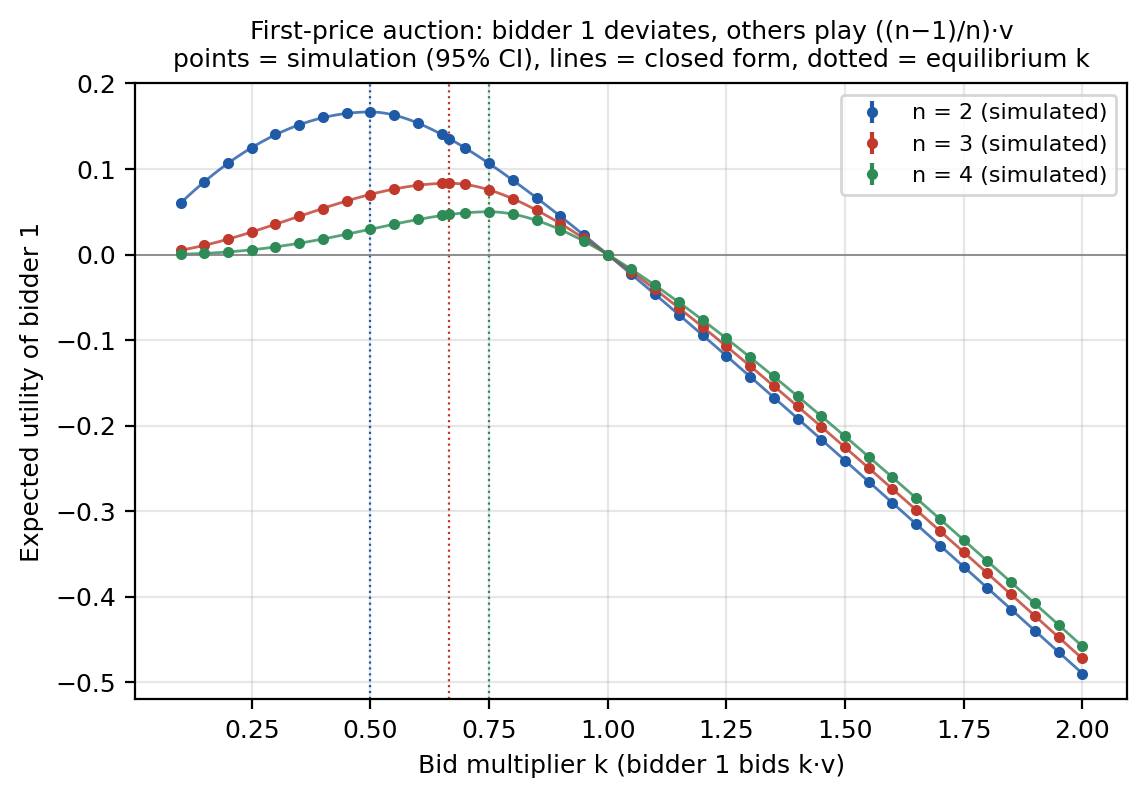
\includegraphics[width=\linewidth]{part2_expected_utility.png}
\end{subfigure}\hfill
\begin{subfigure}{0.46\linewidth}
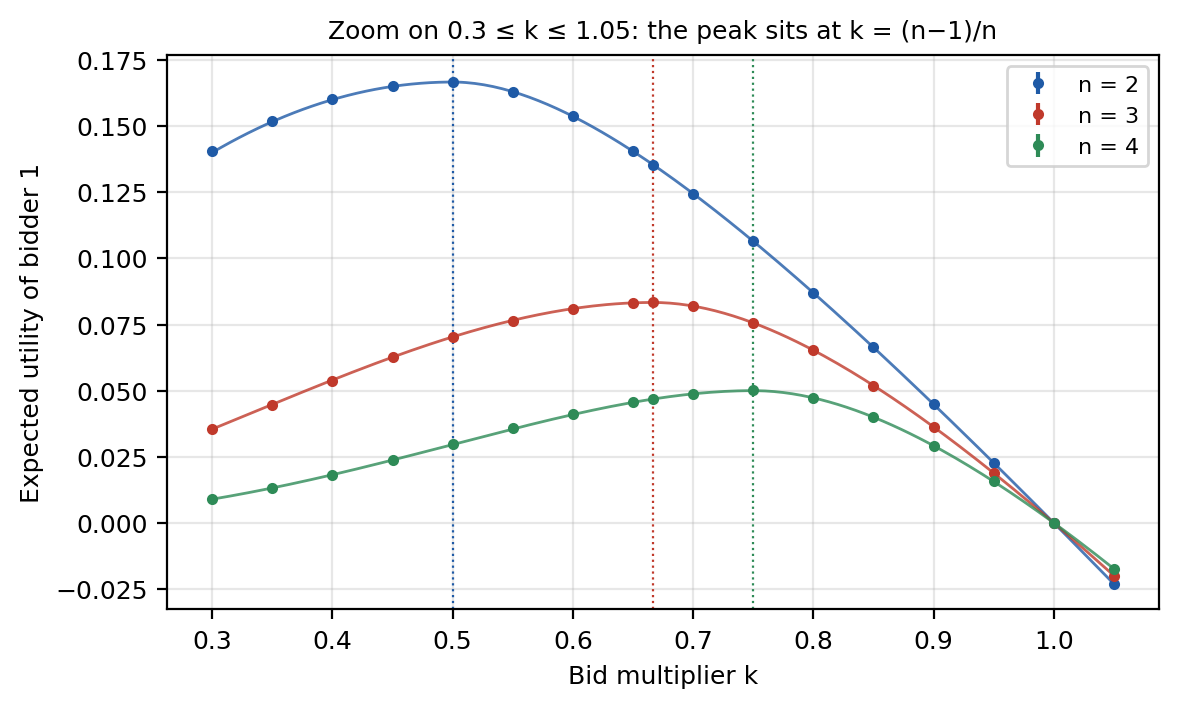
\includegraphics[width=\linewidth]{part2_expected_utility_zoom.png}
\end{subfigure}
\caption{Expected utility of bidder~1 as a function of $k$ for $n=2,3,4$ (left: full grid; right:
zoom on the peak). Points: simulation with 95\% confidence intervals. Lines: closed form. Dotted:
the equilibrium multiplier $(n-1)/n$.}
\label{fig:p2u}
\end{figure}

\begin{table}[!htbp]
\centering
\caption{First-price auction results at selected $k$ (200{,}000 auctions per point). $\hat U$:
simulated expected utility of bidder~1 ($\pm$ 95\% CI half-width $\le 0.0015$). $U$: closed
form. ``Pay less'': share of auctions in which the winning bid exceeds the second-highest bid.
``$>0.01$'': share in which it exceeds it by more than one bid increment. ``Slack'': average
winning bid minus second-highest bid.}
\label{tab:p2}
\small
\begin{tabular}{c c rr c c c c}
\toprule
$n$ & $k$ & $\hat U$ & $U$ & $P(\text{1 wins})$ & Pay less & $>0.01$ & Slack \\
\midrule
2 & 0.25 & 0.1249 & 0.1250 & 0.249 & 1.000 & 0.960 & 0.167 \\
2 & \textbf{0.50} & \textbf{0.1665} & \textbf{0.1667} & 0.499 & 1.000 & 0.960 & 0.167 \\
2 & 0.75 & 0.1065 & 0.1065 & 0.666 & 1.000 & 0.974 & 0.236 \\
2 & 1.00 & 0.0000 & 0.0000 & 0.749 & 1.000 & 0.981 & 0.334 \\
2 & 1.50 & $-0.2409$ & $-0.2407$ & 0.833 & 1.000 & 0.987 & 0.556 \\
2 & 2.00 & $-0.4900$ & $-0.4896$ & 0.874 & 1.000 & 0.990 & 0.792 \\
\midrule
3 & 0.25 & 0.0263 & 0.0264 & 0.047 & 1.000 & 0.965 & 0.200 \\
3 & 0.50 & 0.0701 & 0.0703 & 0.187 & 1.000 & 0.959 & 0.168 \\
3 & \textbf{0.67} & \textbf{0.0834} & \textbf{0.0833} & 0.333 & 1.000 & 0.956 & 0.167 \\
3 & 1.00 & 0.0000 & 0.0000 & 0.555 & 1.000 & 0.971 & 0.241 \\
3 & 1.50 & $-0.2251$ & $-0.2253$ & 0.703 & 1.000 & 0.981 & 0.429 \\
3 & 2.00 & $-0.4720$ & $-0.4722$ & 0.777 & 1.000 & 0.985 & 0.648 \\
\midrule
4 & 0.25 & 0.0055 & 0.0056 & 0.009 & 1.000 & 0.960 & 0.182 \\
4 & 0.50 & 0.0299 & 0.0296 & 0.075 & 1.000 & 0.956 & 0.161 \\
4 & \textbf{0.75} & \textbf{0.0501} & \textbf{0.0500} & 0.250 & 1.000 & 0.948 & 0.150 \\
4 & 1.00 & 0.0000 & 0.0000 & 0.437 & 1.000 & 0.961 & 0.191 \\
4 & 1.50 & $-0.2122$ & $-0.2125$ & 0.624 & 1.000 & 0.974 & 0.356 \\
4 & 2.00 & $-0.4576$ & $-0.4578$ & 0.718 & 1.000 & 0.980 & 0.564 \\
\bottomrule
\end{tabular}
\end{table}

\subsection{How often could the winner have paid less?}
In \emph{every} simulated auction, for every $n$ and $k$, the winner could have paid less and still
won (``Pay less'' $=1.000$ in Table~\ref{tab:p2}). This is structural. Values are continuous, so the
winning bid is strictly above the second-highest bid with probability one, and in a first-price
auction the winner pays its own bid. In a second-price auction this fraction is zero by
construction, because the winner already pays the second-highest bid.

To measure how much money is left on the table, we also count auctions in which the winner could
have bid more than one bid increment ($0.01$) less. That happens in 95--99\% of auctions
(Figure~\ref{fig:p2gap}). At the equilibrium the slack is
$\frac{n-1}{n}(V_{(1)}-V_{(2)})$, where $V_{(1)}$ and $V_{(2)}$ are the two highest values. Two
order-statistics facts give exact predictions:
\begin{itemize}[itemsep=0.1em]
  \item $\mathbb{E}[V_{(1)}-V_{(2)}]=1/(n+1)$, so the mean slack is $\frac{n-1}{n(n+1)}$: $0.167$, $0.167$ and $0.150$ for $n=2,3,4$. We measured $0.167$, $0.167$ and $0.150$.
  \item $P(V_{(1)}-V_{(2)}>t)=(1-t)^n$, so the share with slack above $0.01$ is $(1-0.01\frac{n}{n-1})^n$: $0.960$, $0.956$ and $0.948$. We measured $0.960$, $0.956$ and $0.948$.
\end{itemize}
The slack is smallest near the equilibrium and grows quickly once bidder~1 overbids, since an
overbidding bidder~1 wins with large margins.

\begin{figure}[!htbp]
\centering
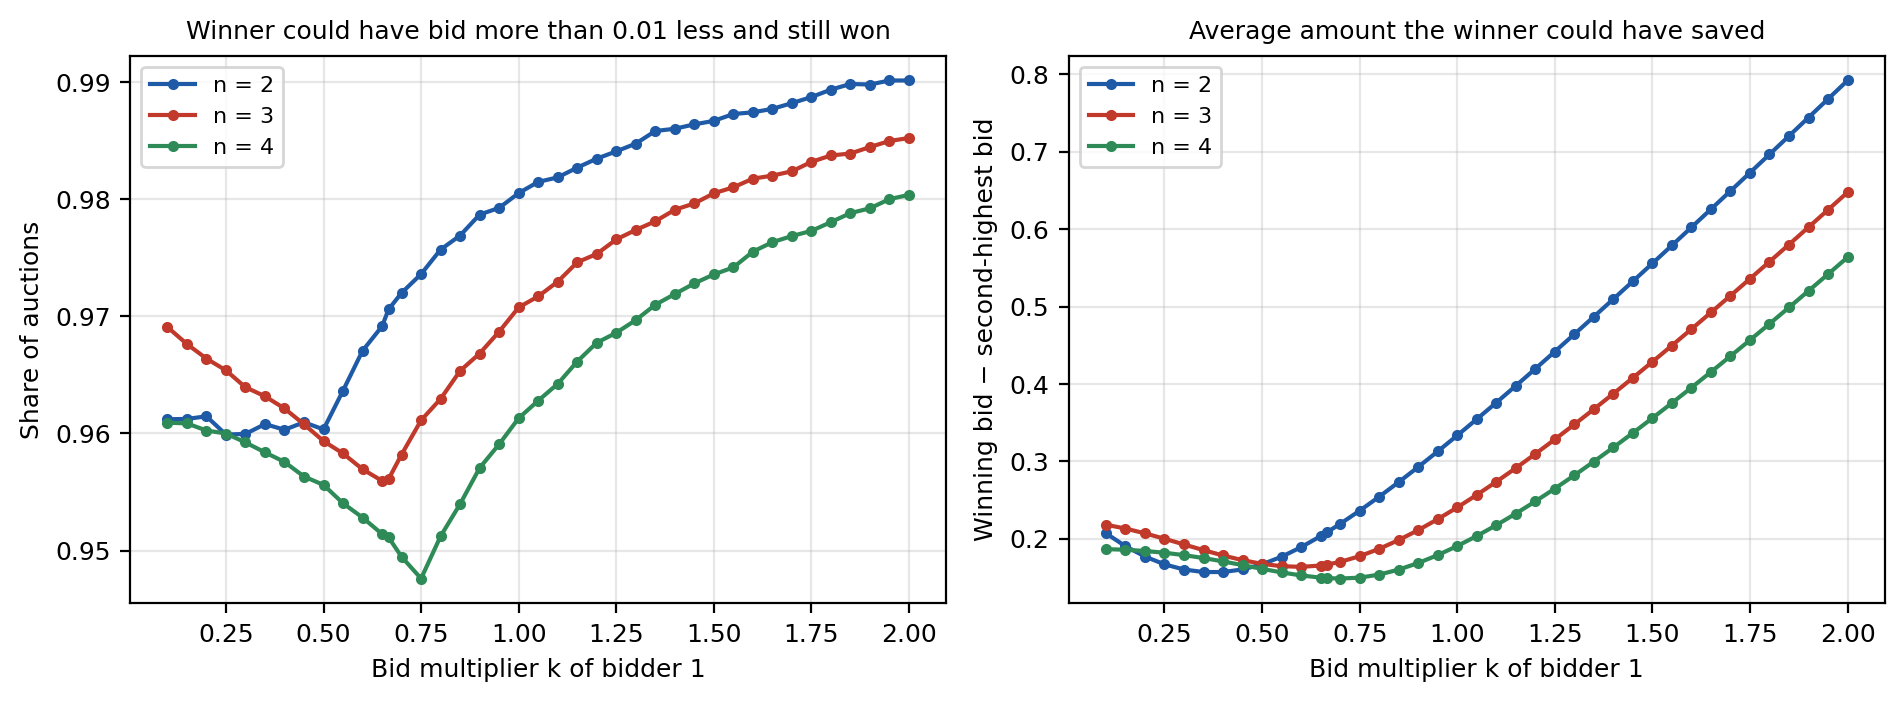
\includegraphics[width=0.95\linewidth]{part2_overpayment.png}
\caption{Left: share of auctions in which the winner could have bid more than $0.01$ less and still
won. Right: average slack (winning bid minus second-highest bid), as a function of bidder~1's
multiplier $k$.}
\label{fig:p2gap}
\end{figure}

%=====================================================================
\section{Part 3: VCG Mechanism for the Cheapest Path}\label{sec:part3}
%=====================================================================
\subsection{Model}
The buyer wants a path from $A$ to $F$ in the undirected network of Figure~\ref{fig:graph}. Each
edge $e$ is owned by a selfish agent whose true cost $c_e$ is private and is incurred only if $e$
is used. Each agent reports a cost $\hat c_e$. The mechanism buys the cheapest path $P^\ast$ under
the reports and pays every edge its Clarke-pivot VCG payment~\cite{nisan2007,shoham2009}:
\begin{equation}\label{eq:vcg}
p_e = C(G\setminus e) - \big(C(G) - \hat c_e\,\mathbf{1}\{e\in P^\ast\}\big),
\end{equation}
where $C(\cdot)$ is the cost of the cheapest path under the reported costs. An off-path edge
receives $p_e=C(G\setminus e)-C(G)=0$. An edge's utility is $p_e-c_e\mathbf{1}\{e\in P^\ast\}$.

Ties between equally cheap paths are broken deterministically: fewer edges first, then the
alphabetical order of the node sequence. Because the network has only six nodes, we compute
cheapest paths exactly by enumerating every simple $A\to F$ path.

\begin{figure}[!htbp]
\centering
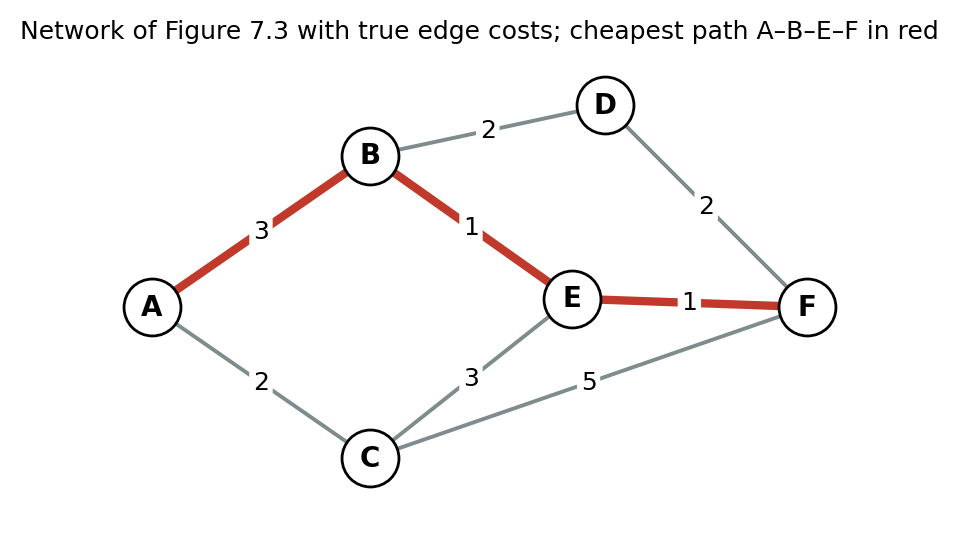
\includegraphics[width=0.62\linewidth]{part3_graph.png}
\caption{The network of Figure~7.3 with its true edge costs. The cheapest path $A$--$B$--$E$--$F$
(cost 5) is shown in red.}
\label{fig:graph}
\end{figure}

\subsection{Reproducing the textbook payments}
With truthful reports, the mechanism selects $A$--$B$--$E$--$F$ with cost $3+1+1=5$.
Table~\ref{tab:vcg} reproduces the payments from the text: $AB$ is paid 4, $BE$ is paid 2,
$EF$ is paid 3, and every other edge is paid 0.

Each on-path payment equals the edge's \emph{critical value}: the highest cost it could report and
still be selected. For example, without $AB$ the cheapest path is $A$--$C$--$E$--$F$ with cost 6.
The other edges on the chosen path cost $1+1=2$, so $AB$ receives $6-2=4$.

The buyer pays $9$ in total for a path that really costs $5$. The premium of $4$ is the
information rent that VCG pays to secure truthful reports.

\begin{table}[!htbp]
\centering
\caption{VCG outcome under truthful reports.}
\label{tab:vcg}
\small
\begin{tabular}{c c c c c c c}
\toprule
Edge & True cost & On $P^\ast$? & $C(G\setminus e)$ & Cheapest path without $e$ & Payment & Utility \\
\midrule
$AB$ & 3 & yes & 6 & $A$--$C$--$E$--$F$ & \textbf{4} & 1 \\
$BE$ & 1 & yes & 6 & $A$--$C$--$E$--$F$ & \textbf{2} & 1 \\
$EF$ & 1 & yes & 7 & $A$--$C$--$F$ & \textbf{3} & 2 \\
$AC$ & 2 & no & 5 & $A$--$B$--$E$--$F$ & 0 & 0 \\
$BD$ & 2 & no & 5 & $A$--$B$--$E$--$F$ & 0 & 0 \\
$CE$ & 3 & no & 5 & $A$--$B$--$E$--$F$ & 0 & 0 \\
$CF$ & 5 & no & 5 & $A$--$B$--$E$--$F$ & 0 & 0 \\
$DF$ & 2 & no & 5 & $A$--$B$--$E$--$F$ & 0 & 0 \\
\midrule
\multicolumn{5}{r}{Total paid by the buyer} & 9 & \\
\bottomrule
\end{tabular}
\end{table}

\subsection{Misreporting costs}
We fix all other reports at their true values and sweep one edge's report $\hat c_e$ over
$0,0.5,\dots,10$. We chose $AB$ (on the path, $c=3$) and $CE$ (off the path, $c=3$). The results
are in Figure~\ref{fig:sweep}.

\paragraph{On-path edge $AB$.}
For any report $\hat c_{AB}\le 4$, $AB$ stays on the chosen path. Its payment is
$6-2=4$ \emph{whatever it reports}, so its utility is constant at $4-3=1$. At $\hat c_{AB}=4$ the
two paths tie at cost 6 and the tie-break keeps $ABEF$. For any report above 4, $ACEF$ becomes
cheaper, $AB$ is dropped, and its utility falls to 0. Reporting a lower cost gains nothing, and
reporting a higher cost can only lose the contract.

\paragraph{Off-path edge $CE$.}
For any report $\hat c_{CE}\ge 2$, $CE$ remains unused and earns 0. Reports below 2 make
$A$--$C$--$E$--$F$ the cheapest path, and $CE$ is then paid $5-(2+1)=2$. But its true cost is 3,
so its utility is $2-3=-1$. Under-reporting to get selected strictly hurts the edge.

\begin{figure}[!htbp]
\centering
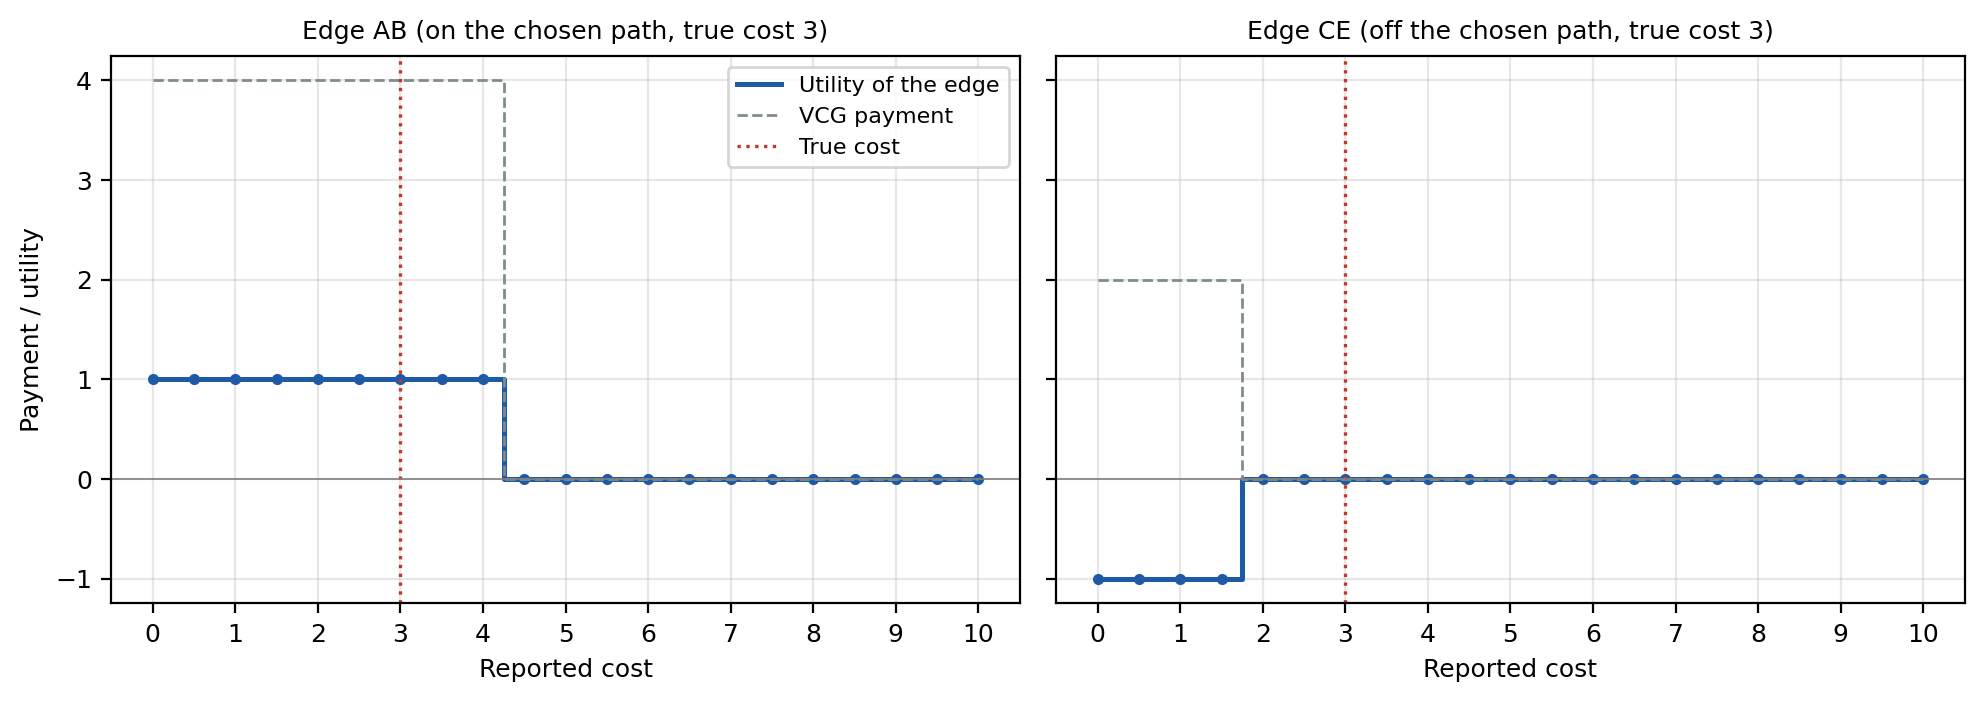
\includegraphics[width=0.97\linewidth]{part3_misreport_sweep.png}
\caption{Utility (solid) and VCG payment (dashed) of an edge as its reported cost varies from 0
to 10, with every other edge truthful. Left: on-path edge $AB$. Right: off-path edge $CE$. The
dotted line marks the true cost.}
\label{fig:sweep}
\end{figure}

\paragraph{All edges.} We repeated the sweep for all eight edges. For every edge, the best utility
over all 21 reports equals its utility under the truthful report (Table~\ref{tab:robust}). No edge
can gain by misreporting, which is the DSIC property of VCG.

\begin{table}[!htbp]
\centering
\caption{Largest utility each edge can reach by misreporting ($\hat c_e\in\{0,0.5,\dots,10\}$),
compared with truthful reporting.}
\label{tab:robust}
\small
\begin{tabular}{l cccccccc}
\toprule
Edge & $AB$ & $AC$ & $BD$ & $BE$ & $CE$ & $CF$ & $DF$ & $EF$ \\
\midrule
Utility when truthful & 1 & 0 & 0 & 1 & 0 & 0 & 0 & 2 \\
Best utility over all reports & 1 & 0 & 0 & 1 & 0 & 0 & 0 & 2 \\
Gain from lying & 0 & 0 & 0 & 0 & 0 & 0 & 0 & 0 \\
\bottomrule
\end{tabular}
\end{table}

%=====================================================================
\section{Implementation}\label{sec:impl}
%=====================================================================
The code is written in Python with NumPy and Matplotlib and is organised as one script per part:
\begin{itemize}[itemsep=0.1em]
  \item \texttt{src/part1\_second\_price.py} implements Parts~1A--1C.
  \item \texttt{src/part2\_first\_price.py} implements Part~2.
  \item \texttt{src/part3\_vcg\_path.py} implements Part~3.
  \item \texttt{src/common.py} holds shared settings.
  \item \texttt{run\_all.py} runs everything.
\end{itemize}
Auction outcomes are computed in vectorised form over all simulated auctions at once. Every
experiment uses a fixed random seed, so running \texttt{python run\_all.py} regenerates exactly the
figures and the numbers reported here. The scripts save every figure to
\texttt{results/figures/} and every number to JSON files in \texttt{results/data/}.

Each simulation is cross-checked against its closed form:
\begin{itemize}[itemsep=0.1em]
  \item Part~1: the expressions in Table~\ref{tab:closed}.
  \item Part~2: Equation~\eqref{eq:fpa} and its extension to $k>\frac{n-1}{n}$.
  \item Part~3: the payments stated in the textbook.
\end{itemize}

%=====================================================================
\section{Conclusion}\label{sec:conc}
%=====================================================================
The simulations confirm the incentive properties that theory predicts for all three mechanisms.
\begin{enumerate}[itemsep=0.2em]
  \item \textbf{Second-price auction.} Truthful bidding maximises bidder~1's utility against every rival strategy, against every fixed rival bid, and with one or two rivals. The bidder needs no model of its opponents, which is exactly what the 9 utility plots show: their peaks all sit at $b=v$.
  \item \textbf{First-price auction.} Truthful bidding is not optimal; it yields zero utility. The best response to equilibrium opponents is to shade the bid to $\frac{n-1}{n}v$, and the simulated optimum matches this for $n=2,3,4$. Because the winner pays its own bid, it could have paid less and still won in every auction, which is the inefficiency that the second-price rule removes.
  \item \textbf{VCG for a cheapest path.} The mechanism reproduces the textbook outcome (path $ABEF$, payments $4,2,3,0$). The misreport sweep shows that an edge's payment does not depend on its own report while it stays selected, so lying can only lose the contract or win it at a loss. The price of this truthfulness is overpayment: the buyer pays 9 for a path that costs 5.
\end{enumerate}

\begin{thebibliography}{9}
\bibitem{vickrey1961} W.~Vickrey. Counterspeculation, auctions, and competitive sealed tenders. \emph{Journal of Finance}, 16(1):8--37, 1961.
\bibitem{clarke1971} E.~H.~Clarke. Multipart pricing of public goods. \emph{Public Choice}, 11:17--33, 1971.
\bibitem{groves1973} T.~Groves. Incentives in teams. \emph{Econometrica}, 41(4):617--631, 1973.
\bibitem{krishna2009} V.~Krishna. \emph{Auction Theory}. Academic Press, 2nd edition, 2009.
\bibitem{nisan2007} N.~Nisan, T.~Roughgarden, \'E.~Tardos and V.~V.~Vazirani (eds.). \emph{Algorithmic Game Theory}. Cambridge University Press, 2007.
\bibitem{shoham2009} Y.~Shoham and K.~Leyton-Brown. \emph{Multiagent Systems: Algorithmic, Game-Theoretic, and Logical Foundations}. Cambridge University Press, 2009.
\end{thebibliography}

\end{document}
